\documentclass[12pt]{article}

\usepackage{listings} % Code listings
\usepackage{verbatim} % For comments
\usepackage{setspace} % For double spacing
\usepackage{cite}  % For citations
\usepackage{url} % For url in citations...maybe
\usepackage{tabularx}
\usepackage{graphicx} % For graphics
\usepackage{multicol}
\usepackage{epstopdf}
\usepackage{enumitem} % Reduce enumerate spacing
\usepackage{hyperref} % \href{}

\doublespacing
\begin{document}

\title{A Replicable and Extensible Comparison of QUIC and TCP}
\author{Henry Baxter and Liam Simmons\\
		University of Victoria}
\date{\today}

\maketitle

\begin{abstract}
	Quick UDP Internet Connections (QUIC) is a transport protocol, first implemented by Google in 2013. Since then, it has seen rapid development over many version numbers. Analysis of QUIC is relatively limited, as compared to TCP, the protocol it is largely meant to replace. We set out to create a replicable and extensible method of comparison of the QUIC and TCP protocols. Running evaluation with 540 distinct combinations of testing parameters, over three distinct network environments, we found that QUIC outperforms TCP in nearly every situation when the Internet is included. On a single VLAN, TCP edges out QUIC. Overall, QUIC is more suitable for fast initial user response times, which reflects typical web use.
\end{abstract}

\section{Introduction}
\label{introduction}

QUIC (Quick UDP Internet Connections) is a new transport protocol, first implemented by Google in 2013. QUIC is designed to be optimized for HTTP traffic; it has several features that are similar to TCP+TLS, but is built on top of UDP. One major difference between TCP and QUIC is that QUIC is implemented in the userspace\cite{quicLayout}, whereas TCP exists within the OS kernel. While changes to TCP can take years to see wide-spread deployment, since QUIC exists as a self-contained protocol, QUIC sees rapid development. Further, QUIC is an encrypted protocol. This prevents QUIC from being tampered with by middleboxes and legacy systems, extending QUIC's ability to be quickly developed. 
% Citation for backwards incompatible changes every 6 weeks?

While these features allow QUIC to see swift development, they in turn make analysis of the protocol very difficult. Following the work of Kakhki, et al.\cite{Kakhki:2017:TLL:3131365.3131368}, we firstly replicate the work of Kakhki and verify their conclusions. We additionally modify their methodology to allow for replicability and tracking of future QUIC versions.

Comparison of QUIC and TCP is done in three testing environments. One, a local client makes requests to an EC2 instance that acts as the QUIC and TCP server, with an additional EC2 instance used to shape network traffic. The second testing environment exists entirely on an Amazon VLAN; one EC2 instance acts as a desktop computer, with two other EC2 instances acting as a router and server, as above. The third testing environment is similar to the second, with the exception that the EC2 Desktop is at a different physical location than the router and server. Parallel requests are made to the QUIC and TCP server, with variations in pages requested, as well as varying network conditions.

Our results show that QUIC outperforms TCP for nearly all variables tested from the local client. The one case where TCP outperforms QUIC from the local client is for very large numbers of objects. This finding is consistent with Kakhi, et al. For testing done within the Amazon VLAN, TCP slightly outperforms QUIC. This may suggest optimizations for TCP within AWS. Testing in the third scenario was done as an attempt to explain lack of QUIC performance in the same VLAN. Results in this scenario are similar to those with a local client.

In Section \ref{background}, we give a brief overview of the QUIC protocol, and the features that allow for improved performance over TCP. We also present related work on the analysis of QUIC. In Section \ref{methods}, our testbed and methodology are described in detail. In Section \ref{data_results}, the aggregation of our data is presented, and is discussed in detail. The conclusions of our findings are presented in Section \ref{conclusions}.

\section{Background}
\label{background}

\subsection{What is QUIC?}
\label{background:quic}

QUIC is a new transport protocol, first implemented by Google in 2013. Far from being an experimental protocol, QUIC is supported by all Google services, including the Chrome browser, YouTube app, and Google Search app on Android\cite{Langley:2017:QTP:3098822.3098842}. By Google's own estimation, in 2017 QUIC made up 7\% of Internet traffic\cite{Langley:2017:QTP:3098822.3098842}.

\begin{figure}
\centering
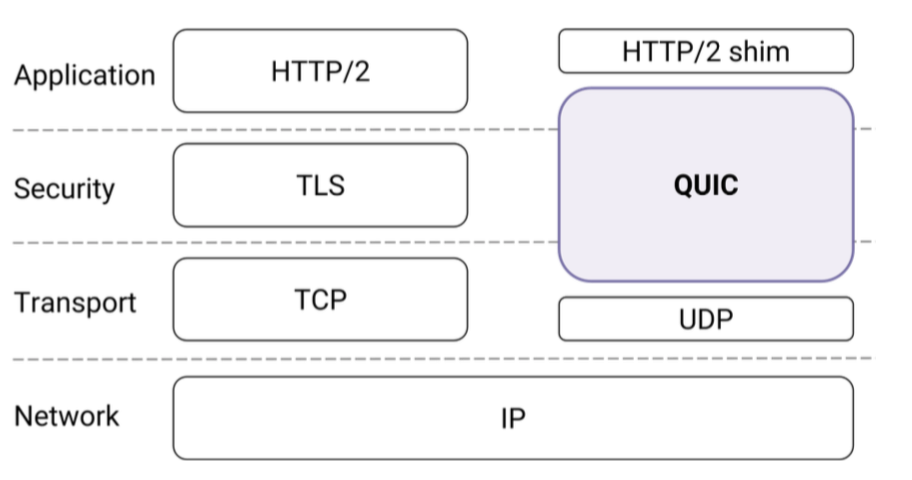
\includegraphics[scale=.25]{images/quic_stack.png}
\caption{QUIC in the traditional HTTPS stack. Image credit \cite{Langley:2017:QTP:3098822.3098842}}
\label{fig:quic_stack}
\end{figure}

QUIC is designed to optimize HTTPS traffic. It is functionally equivalent to TCP+TLS+HTTP/2\footnote{For the purpose of this report, \emph{TCP} will refer to \emph{TCP+TLS+HTTP/2}}, but is built on top of UDP. QUIC exists entirely within the userspace, which allows rapid evolution of the protocol. QUIC has several features that allow it to perform better than TCP, including:
\begin{itemize}
	\item \textbf{Reduced latency for connection establishment}
	\item \textbf{Stream multiplexing without head-of-line blocking}
	\item \textbf{Improved congestion control and loss recovery}
\end{itemize}

\textbf{Reduced Connection Latency:} QUIC combines both the transport and cryptographic handshake to reduce connection latency. For new connections, QUIC requires only 1-RTT to establish a connection\footnote{When there is no version negotiation}. This is one and two RTTs faster than TCP+TLS1.3 and TCP+TLS1.2, respectively\cite{7867726}. When a connection has been previously established, QUIC requires 0-RTT to re-establish the connection, by caching cryptographic values of the server on the client side.

\begin{figure}
\centering
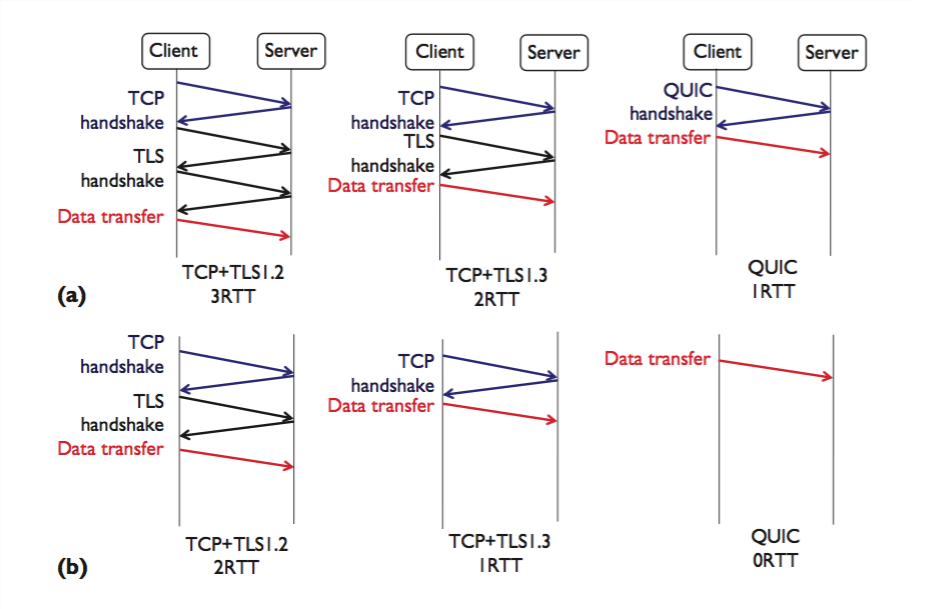
\includegraphics[scale=.3]{images/QUIC_TCP_RTT.png}
\caption{Handshake RTT of different protocols for (a) first time connection establishment and (b) subsequent connections. Image credit \cite{7867726}}
\label{fig:RTT}
\end{figure}

\textbf{Stream Multiplexing:} QUIC is designed for multiplexed operation; it allows multiple streams to exist for each connection. Within a QUIC stream, lost packets generally only affect that stream. Other streams can continue to make progress. QUIC can also abandon streams without concern. While HTTP/2 also features stream multiplexing, it exists on top of TCP's single byte-stream abstraction. When a segment is lost, all further segments are blocked until a retransmission occurs. QUIC reduces latency of retransmission by avoiding head-of-line blocking\cite{quicLayout}.

\begin{figure}
\centering
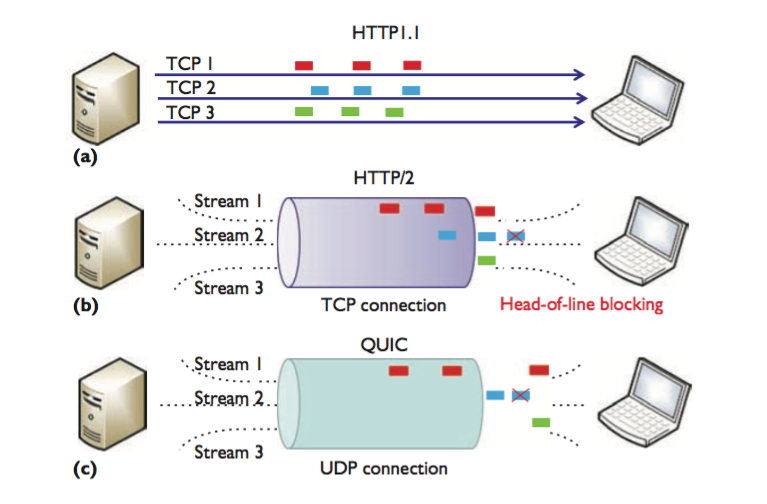
\includegraphics[scale=.4]{images/QUICmulti.png}
\caption{Multiplexing comparison of (a) HTTP1.1 (b) HTTP/2 and (c) QUIC. Image credit \cite{7867726}}
\label{fig:multiplex}
\end{figure}

\textbf{Improved Congestion Control and Loss Recovery:} For all packets, QUIC uses unique, monotonic sequence numbers. This allows QUIC to easily differentiate original from retransmitted packets, thus avoiding retransmission ambiguity found with TCP. QUIC ACK packets also explicitly carry the delay of packet reception to acknowledgment being sent, which allows QUIC to more accurately calculate RTT, and therefore further refine congestion control\cite{quicLayout}.

\subsection{Related Work}
\label{background:related}
As stated above, Kakhki et al. provides a starting point for our analysis. To the best of our knowledge, it is the most comprehensive comparison of QUIC and TCP to date. Further papers that provide analysis of QUIC performance include:

\begin{itemize}
	\item How Quick is QUIC?\cite{Megysei:2016:HQQ}
	\item HTTP over UDP: An Experimental Investigation of QUIC\cite{Carlucci:2015:HOU}
	\item Does QUIC make the web faster?\cite{Biswal:2016:DQM}
	\item Evaluation of QUIC in Web Page Performance\cite{Das:2014:EQW}
\end{itemize}

\section{Motivation}
\label{motivation}
QUIC is a rapidly evolving protocol, that is used for all Google services. As public analysis of QUIC is extremely limited as compared to TCP, it is vitally important that a deeper understanding of QUIC performance characteristics be both publicly accessible and replicable. With an experimental design focused on replicability and extensibility, we aim to provide both a comparative analysis of QUIC and TCP, as well as a model for future comparisons. In this way, future changes to the QUIC protocol can be quickly and efficiently tracked and analyzed.

\section{Methods}
\label{methods}
We now describe the methods used to compare the TCP and QUIC protocols.

% Which processor on local desktop? Which NGINX version? Is QUIC source accurate as described?
\subsection{Testbed}
Evaluation was performed in three different network environments, as shown in figure \ref{fig:network}.

The server and remote desktops run on Amazon EC2 T2.Large (Kernel 4.4.0-1054-aws, Ubuntu 16.04, 8 GB memory, Intel Xeon 3.0GHz\footnote{The T2 EC2 instance uses `burstable' CPU, so clock speed is \emph{up to} 3.0 GHz}).The router runs on Amazon EC2 T2.micro (Kernel 4.4.0-1054-aws, Ubuntu 16.04, 1 GB memory, Intel Xeon 3.3 GHz\footnote{Again, \emph{up to} 3.3 GHz}). The EC2 router and server are located on ec2-east1. One EC2 desktop is on ec2-east1 (as in fig. \ref{fig:network} (b)), and another on ec2-west1 (as in fig. \ref{fig:network} (c)).

The local client is a desktop (macOS High Sierra 10.13.4, 32 GB memory, Intel Xeon 3.5 GHz).

All clients run Google Chrome (ver. 65.0.3325.181 (Official Build) (64-bit)). The server supports HTTP/2 over TCP via NGINX 1.10.3 with OpenSSL 1.0.2g and TLS SNI, and over QUIC via the QUIC standalone server, as provided with the Chromium source code at commit 902d73b.

\begin{figure}
\begin{tabular}{c c}
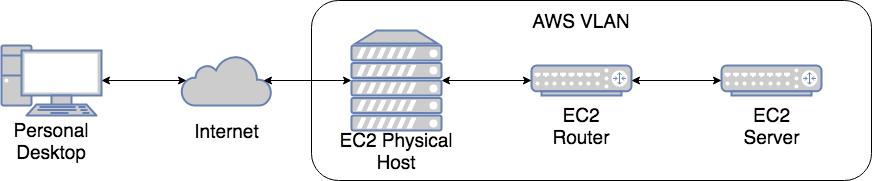
\includegraphics[scale=.25]{images/local.png} & 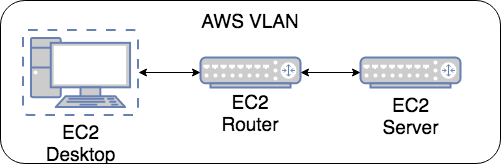
\includegraphics[scale=.25]{images/aws.png}\\
~ & ~ \\
(a) & (b) \\
~ & ~ \\
\multicolumn{2}{c}{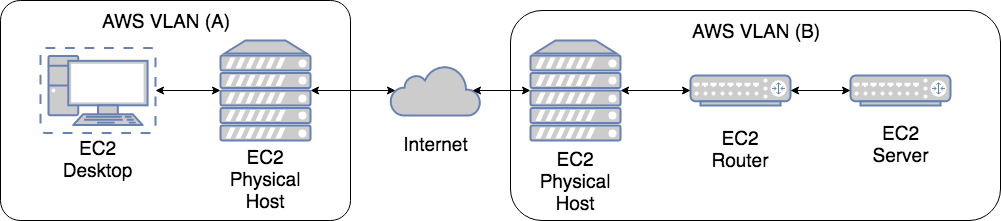
\includegraphics[scale=.25]{images/aws_inet.png}} \\
~ & ~ \\
\multicolumn{2}{c}{(c)} \\
\end{tabular}
\caption{Testbed setup for local (a), EC2 on same VLAN (b) and EC2 on separate VLAN (c)}
\label{fig:network}
\end{figure}

\subsection{Testing Workflow}
Since a major objective of this work was the reproducibility and extensibility of the testing protocol, we go into it in some detail here. Despite significant capabilities, it was achieved in 500 lines of idiomatic Python and 100 lines of BASH shell code. The majority of the work can be seen on GitHub at \url{https://github.com/henrybaxter/csc466/blob/master/main.py} and the router traffic shaping tool here \url{https://github.com/henrybaxter/csc466/blob/master/set_router.sh}.

Configuration files are written in TOML format, a subsection of which is shown in \ref{fig:config} to demonstrate the ease of adding or removing test cases. Under the \textit{treatment} heading are treatment defaults, and under the \textit{variations} heading are a list of values to vary for whichever dimension is desired, and under dual-variations one can have an unlimited number of two dimensional treatments for the production of heatmaps or other insightful data analysis.

\begin{figure}
\begin{lstlisting}
[treatment]
	delay-time = 20
	delay-jitter = 5
	delay-correlation = 25
	delay-distribution = 'normal'
	# Gilbert-Elliot packet loss model
	loss-p = 0.0
	loss-r = 100.0
	loss-h = 100.0
	loss-k = 0.0
	corrupt-percent = 0.0
	corrupt-correlation = 25
	duplicate-percent = 0.0
	duplicate-correlation = 25
	rate-limit = 50.0
	object-count = 5
	object-size = 10

[variations]
	rate-limit = [1.0, 5.0, 10.0, 25.0, 50.0]
	object-count = [5, 10, 50, 100, 200]
	object-size = [5, 10, 100, 200, 500, 1000]
	loss-p = [0.0, 1.0, 2.0, 3.0, 5.0]
	corrupt-percent = [0.0, 1.0, 2.0, 3.0, 5.0, 10.0, 15.0]
	duplicate-percent = [0.0, 1.0, 2.0, 3.0, 5.0, 10.0, 15.0]
	delay-time = [20, 50, 100, 150, 200]
	delay-jitter = [5, 20, 40, 60, 80, 100]

[[dual-variations]]

	axis1 = 'delay-time'
	axis2 = 'delay-jitter'
	values = [[100, 20], [200, 20]]
\end{lstlisting}
\label{fig:config}
\caption{Configuration TOML}
\end{figure}

The testing program is given a configuration file as a command line argument. It follows a basic algorithm:

\begin{enumerate}[topsep=0pt,itemsep=-1ex,partopsep=1ex,parsep=1ex]
	\item Generate treatment details for every variation and dual variation listed
	\item Launch Chrome processes and connect to their remote debugging inteface
	\item Start an SSH session with the remote router running on AWS
	\item Run each treatment
	\begin{enumerate}[topsep=0pt,itemsep=-1ex,partopsep=1ex,parsep=1ex]
		\item Configure the remote router with the correct network variation parameters
		\item Configure the local Chrome instance with the correct request parameters
		\item Fire the request and return the resulting timing information
	\end{enumerate}
	\item Save and aggregate the results as both JSON and CSV
\end{enumerate}

During the course of testing a variety of information is provided on screen and logged permanently, including the estimated time to complete the given tests.

Once testing is complete, charts are automatically generated using standard Python scientific computing tools Panda and Seaborn (based on Matplotlib). Adding new chart types is a matter of writing a few line function as a form of plugin.

\subsection{Testing Variables}
Various treatments of network conditions were evaluated for each of the protocols. Parallel instances of Chrome were launched on either a local machine, or an EC2 instance. Treatments were generated from a configuration file, the variations are shown in figurte \ref{test_variables}. When a treatment is run, the test environment is automatically configured. Requests are initiated programmatically and page load time is captured for multiple runs. For each treatment, 100 iterations are performed of each protocol.

Network shaping was performed at the EC2 router using tc htb and qdisc.
% Going off of config file as of 04/11/18:46...update if there are others missing
\begin{figure}
\centering
\begin{tabular}{c|c}
	Parameter	&	Values tested 	\\\hline
	Rate Limit (Mbit) 	&	1, 5, 10, 25, 50	\\
	Object Size (KB)	&	5, 10, 100, 200, 500, 1000	\\
	Object Count &	5, 10, 50, 100, 200	\\
	Packet Loss (\%)	&	0, 1, 3, 5	\\
	Packet Corruption (\%) & 0, 1, 2, 3, 5, 10*, 15* \\
	Packet Duplication (\%) & 0, 1, 2, 3, 5, 10, 15 \\
	Packet Delay (ms)		&	20, 50, 100, 150, 200	\\
	Packet Jitter (ms)		& 5, 20, 40, 60, 80, 100 \\
\end{tabular}
\caption{Test Variables (*only for the EC2 instance on the same VLAN)}
\label{test_variables}
\end{figure}

\section{Data and Results}
\label{data_results}

Ninety treatments as detailed in Figure \ref{test_variables} were run for TCP/HTTP2 and QUIC, from three locations, with 100 iterations each, giving a total of 54,000 requests. These results were aggregated down to the 540 distinct situations with their mean and standard deviation recorded. The raw results and these aggregations are available on request.

We present a selection of charts, comparing the three environments horizontally in every case.

\begin{figure}[h]
\centering
\begin{tabular}{c c c}
	Local Desktop & Same VLAN & Cross-Continent EC2 Instance \\
	\includegraphics[width=.33\textwidth]{{plots/local/rate-limit}.eps} &
	\includegraphics[width=.33\textwidth]{{plots/ec2-east1/rate-limit}.eps} &
	\includegraphics[width=.33\textwidth]{{plots/ec2-west1/rate-limit}.eps} \\
\end{tabular}
\caption{Comparing effect of rate limit}
\label{figs:rate_limit}
\end{figure}

In Figure \ref{figs:rate_limit} we see that for a local desktop consumer on a typical Internet connection, we can expect QUIC to outperform TCP/IP in every case, but maximally in the 5-25 megabit range. QUIC does not outperform TCP/IP when the desktop is on the same VLAN and in the same physical location in the AWS cloud.

By showing that an EC2 instance in a different physical location and on a different VLAN has performance similar to a consumer desktop, we see that there is some network condition or optimization in play that is not peculiar to EC2, Linux, the Chrome Linux build, or the AWS cloud in general. Extensive investigation with iperf and varying network parameters as in the following data have not yielded an explanation for this discrepancy.


\begin{figure}[h]
\centering
\begin{tabular}{c c c}
	Local Desktop & Same VLAN & Cross-Continent EC2 Instance \\
	\includegraphics[width=.33\textwidth]{{plots/local/loss-p}.eps} &
	\includegraphics[width=.33\textwidth]{{plots/ec2-east1/loss-p}.eps} &
	\includegraphics[width=.33\textwidth]{{plots/ec2-west1/loss-p}.eps} \\
\end{tabular}
\caption{Comparing effect of packet loss}
\label{figs:packet_loss}
\end{figure}

In Figure \ref{figs:packet_loss} using the Gilbert-Ellison model of packet loss in the netem model, we see that QUIC has a more robust response to bad state transitions of up to 5\%. This is inconsistent with the findings of Kakhi, et al. The model of packet loss used by Kakhi was a simple uniform drop, which could account for the difference.

\begin{figure}[h]
\centering
\begin{tabular}{c c c}
	Local Desktop & Same VLAN & Cross-Continent EC2 Instance \\
	\includegraphics[width=.33\textwidth]{{plots/local/duplicate-percent}.eps} &
	\includegraphics[width=.33\textwidth]{{plots/ec2-east1/duplicate-percent}.eps} &
	\includegraphics[width=.33\textwidth]{{plots/ec2-west1/duplicate-percent}.eps} \\
\end{tabular}
\caption{Comparing effect of packet duplication}
\label{figs:packet_duplication}
\end{figure}

Packet duplication has a negligible impact on either protocol as show in Figure \ref{figs:packet_duplication}. This makes sense, since duplicate packets are easily disgarded by either protocol, and can in fact decrease the overall response time if there is some packet jitter and unused bandwidth, since packets are effectively racing to be first. This may explain the slight drop in page load time as duplication occurs.

\begin{figure}[h]
\centering
\begin{tabular}{c c c}
	\includegraphics[width=.33\textwidth]{{plots/local/corrupt-percent}.eps} &
	\includegraphics[width=.33\textwidth]{{plots/ec2-east1/corrupt-percent}.eps} &
	\includegraphics[width=.33\textwidth]{{plots/ec2-west1/corrupt-percent}.eps} \\
\end{tabular}
\caption{Comparing effect of packet corruption}
\label{figs:packet_corruption}
\end{figure}

The packet corruption charts in Figure \ref{figs:packet_corruption} have different domains. The tests run on the same VLAN were able to complete with very high corruption rates of 10\% and 15\%, whereas those run across the Internet simply failed. However despite this visual inconsistency, the impact of random errors in packets is strongest on TCP/IP. The intuitive explanation for this is the greater reliance TCP/IP has on individual packets, as seen in the packet loss charts of Figure \ref{figs:packet_loss}. Further, it is important to recognize that despite QUIC being built on top of UDP which has no error detection, QUIC itself is capable of handling very high error rates.

\begin{figure}[h]
\centering
\begin{tabular}{c c c}
	Local Desktop & Same VLAN & Cross-Continent EC2 Instance \\
	\includegraphics[width=.33\textwidth]{{plots/local/delay-time}.eps} &
	\includegraphics[width=.33\textwidth]{{plots/ec2-east1/delay-time}.eps} &
	\includegraphics[width=.33\textwidth]{{plots/ec2-west1/delay-time}.eps} \\

	\includegraphics[width=.33\textwidth]{{plots/local/delay-jitter}.eps} &
	\includegraphics[width=.33\textwidth]{{plots/ec2-east1/delay-jitter}.eps} &
	\includegraphics[width=.33\textwidth]{{plots/ec2-west1/delay-jitter}.eps} \\
\end{tabular}
\caption{Comparing effect of packet loss, duplication, delay, and jitter}
\label{figs:packet_timing}
\end{figure}

Adjusting delay time effectively doubles RTT since delays have an impact at both ingress and egress of the router. The jitter values have an impact beyond the typical jitter one might experience in a VOIP conversation, and in fact were not chosen for their primary effect. By increasing jitter beyond the delay time, packet reordering is introduced. Figure \ref{figs:packet_timing} shows the standard result that for lossless situations the desktop on the same VLAN has higher TCP/IP performance, while QUIC outperforms in the Internet setting. With increasing RTT, jitter, and its secondary effect packet reordering, there is a linear impact on both QUIC and TCP/IP with remarkably similar slopes.

\begin{figure}[h]
\centering
\begin{tabular}{c c c}
	Local Desktop & Same VLAN & Cross-Continent EC2 Instance \\
	\includegraphics[width=.33\textwidth]{{plots/local/object-count}.eps} &
	\includegraphics[width=.33\textwidth]{{plots/ec2-east1/object-count}.eps} &
	\includegraphics[width=.33\textwidth]{{plots/ec2-west1/object-count}.eps} \\

	\includegraphics[width=.33\textwidth]{{plots/local/object-size}.eps} &
	\includegraphics[width=.33\textwidth]{{plots/ec2-east1/object-size}.eps} &
	\includegraphics[width=.33\textwidth]{{plots/ec2-west1/object-size}.eps} \\
\end{tabular}
\caption{Comparing effect of object size and count}
\label{figs:objects}
\end{figure}

Figure \ref{figs:objects} shows results that are inconsistent with Kakhi, and also with results that were gathered initially with this work. In particular, QUIC has significantly higher page load times for object counts between 10 and 50 even in the non-VLAN case, and in all environments for object sizes larger than approximately 50kb.

A significant change in methodology near the end of this work led to interacting with the linux tc-netem module in a different way.

\begin{figure}
\begin{lstlisting}[basicstyle=\tiny]
tc qdisc add dev ifb0 root handle 1: htb default 10
tc class add dev ifb0 parent 1: classid 1:1 htb rate 1000mbit
tc class add dev ifb0 parent 1:1 classid 1:10 htb rate 1000mbit
tc class add dev ifb0 parent 1:1 classid 1:5 htb rate ${RATE_LIMIT}mbit ceil ${RATE_LIMIT}mbit
tc filter add dev ifb0 protocol ip parent 1: prio 1 u32 match ip sport 23 0xfff flowid 1:5
tc filter add dev ifb0 protocol ip parent 1: prio 1 u32 match ip sport 80 0xfff flowid 1:5
tc filter add dev ifb0 protocol ip parent 1: prio 1 u32 match ip sport 443 0xfff flowid 1:5
tc filter add dev ifb0 protocol ip parent 1: prio 1 u32 match ip sport 5001 0xfff flowid 1:5
tc qdisc add dev ifb0 parent 1:5 handle 10: netem  \
	limit 100000 \
	delay ${DELAY_TIME}ms ${DELAY_JITTER}ms ${DELAY_CORRELATION}% distribution ${DELAY_DISTRIBUTION} \
	loss gemodel ${LOSS_P} ${LOSS_R} ${LOSS_1H} ${LOSS_1K} \
	corrupt ${CORRUPT_PERCENT}% ${CORRUPT_CORRELATION}% \
	duplicate ${DUPLICATE_PERCENT}% ${DUPLICATE_CORRELATION}%
\end{lstlisting}
\caption{Excerpt of router configuration showing netem interaction}
\label{figs:netem}
\end{figure}

Figure \ref{figs:netem} shows that netem is given arguments for delay, loss, corruption, and duplication regardless of what these arguments are. In particular, it is not clear from the netem model if, for example, setting corruption and corruption correlation to zero is identical to not setting it at all. This would be an excellent place to look for the discrepancy, and could be determined shortly either empirically or by inspection of the netem source code.

Another possible explanation is that the QUIC server, as described in the Chromium source code, is not at all meant to be production quality or performant. Unfortunately there are no production QUIC servers written by Google that are open source, however there are third party projects such as Caddy, which uses a library written in Golang for QUIC. This is also unlikely to be as performant as NGINX. In particular, it is not clear without further inspection of the QUIC experimental server source code how multiple QUIC streams are threaded, particularly if they are requesting disparate files on the hard drive. This is another avenue for investigation.

\section{Conclusions}
\label{conclusions}
By building a framework and testing harness that is highly modular and configurable that generates actionable and visual results on the fly, we have met the goal of building a replicable and extensible comparison of QUIC. In the process of running tests we have found a number of intriguing results that demand further experimentation and analysis. In particular, the QUIC protocol suffers during intradatacenter communication on AWS, and when handling very large or very high numbers of objects.

However, it is clear at this point that QUIC is more suitable for fast initial user response times in the majority of web use cases. Further exploration and elucidation of these results will require minimal setup and zero programming effort by a third party, as full source code and documentation is available online on GitHub at \url{https://github.com/henrybaxter/csc466}.

\appendix

\clearpage

\section{Contributions}
The following is a summary of the contributions of each team member:

\begin{tabularx}{\textwidth}{X|X}
Henry:	&	Liam:	\\ \hline
\textbullet Wrote the project proposal	&	\textbullet Set up website	\\
\textbullet Website Updates				&	\textbullet Website Updates	\\
\textbullet	Set up of QUIC, TCP Servers	&	\textbullet	Image creation for testing	\\
\textbullet	Writing of Python code for programmatic testing	&	\textbullet	Writing of Python code for page generation \\
\textbullet Running of tests			&	\textbullet Poster creation, outline \\
\textbullet Poster content 				&	\textbullet Poster content \\
\textbullet Overall data collection		&	\textbullet	Report outline \\
\textbullet	Report content 				&	\textbullet Report content \\
\end{tabularx}

\bibliography{bibliography}{}
\bibliographystyle{unsrt}
\end{document}
